\chapter{Component compilation}
This chapter looks closely into a phase of the problem solving that can be regarded as a preparation step. The way Symfony Components are packed into NuGet packages and the tools that help to automatize the process are discussed here. 

At first, a brief introduction into MSBuild tool will be provided as it forms a required knowledge for further understanding. After that, we will present more detailed overview of solution design. Description of various configuration files that accompany the build process will follow, ending the chapter with a section about implemented automatization of the whole Components compilation.

\paragraph{} The source code for the NuGet packages of Symfony components provided with the project can be found under the \texttt{Peachpied.Symfony/Components/4.2.3} directory. It was included in the project due to certain modifications that distinguish it from the one acquired by the \texttt{composer require "[name]:[version]"} command. More about these changes and their purpose will be discussed later on. For clarification, when speaking of a certain package folder or a \texttt{vendor} directory in the following text, those in this particular directory are meant unless stated otherwise. Moreover, custom notation \texttt{\{* ... *\}} will be used in examples on places where the thought behind the expression is of higher importance than actual implementation.


\section{MSBuild}
When a .NET project is compiled, MSBuild build system takes the configuration stored in \texttt{.[projectType]proj} file that is associated with the project and performs the compilation \citep{microsoft.docs}. The project type by convention reflects the actual extension of the file and is used in order to increase their understandability \citep{microsoft.docs}. Some of generally used extensions are \texttt{.csproj} for C\# projects, \texttt{.vbproj} for Visual Basic .NET projects, and \texttt{.msbuildproj} for projects not tied to any specific language. The \texttt{.msbuildproj} file extension is also used by Peachpie Software Development Kit (SDK). In addition, \texttt{.targets} and \texttt{.props} extensions are recognized as reusable project files that can be imported to other project files \citep{microsoft.docs}. Regardless the final extension and usage, all of the \texttt{.[projectType]proj} files are XML files that adhere to the MSBuild XML schema \citep{microsoft.docs}.

The basic syntax of MSBuild XML schema uses properties and items as a way of passing information to tasks. Where properties are name-value pairs, items are collections of values and can contain attributes. There are many additional differences between properties and items such as their typical usage, the way they are passed to tasks or the way they are processed. MSBuild reserves some property names as a mean of storing information about the project file \citep{microsoft.docs}, those are for example \texttt{MSBuildThisFileDirectory} or \texttt{MSBuildProjectDirectory}. Properties can be referenced by using the \texttt{\$([propertyName])} notation, items by \texttt{@([ItemName])}. Furthermore, new items and properties can be defined by using their name as a child element of either \texttt{PropertyGroup} for properties or \texttt{ItemGroup} for items.

Aside from that, MSBuild provides a way to modify compilation process by hooking custom targets into the build order. Target is a set of tasks, functional units providing certain actions, represented by a \texttt{Target} element. On the .NET project compilation, a list of default targets is sequentially executed performing each target's actions or skipping them based on provided conditions, resulting in the project's compilation. MSBuild has a built-in collection of tasks providing basic actions such as \texttt{Delete}, \texttt{Copy} or \texttt{Message}. In addition to, custom tasks can be registered from assemblies via the \texttt{UsingTask} element. We can include custom tasks written as .NET class libraries that will provide us with the required missing functionalities. Such class only needs to either implement the \texttt{Microsoft.Build.Framework.ITask} interface or inherit from the \texttt{Microsoft.Build.Framework.Task} class and define an \texttt{Execute} method returning a \texttt{boolean} value. Task's input parameters are supplied through attributes and correspond to the .NET properties in the class definition. Output parameters of the task are created by marking selected .NET properties with the \texttt{[Output]} attribute. These can be collected after task's execution with the \texttt{Output} subelements which perform mapping from .NET property to either MSBuild item or property.


\section{Solution design}
For each library, we need to create a project, more precisely, we need a \texttt{.msbuildproj} file that will be supplied to the MSBuild task. Initially, to include Peachpie compiler we need to set the \texttt{Sdk} attribute of the root \texttt{Project} element to \texttt{Peachpie.NET.Sdk/[version]}. This way, the properties and the targets used by Peachpie compiler will be imported into the project. The second step is to set the \texttt{GeneratePackageOnBuild} property to true in order for MSBuild to output a NuGet package. Then we need to specify files that are to be compiled, excluded and copied to the output package in a form of static content. For this purpose, items \texttt{Compile} and \texttt{Content}, and their attributes \texttt{Include}, \texttt{Exclude} and \texttt{Remove} can be used. When MSBuild copies static files to the output, it by default preserves the structure the files are located in. As the NuGet packages will be used and referenced from the user defined content of the project, it is preferable to place all the \texttt{.msbuildproj} files for each project to parent directory of \texttt{vendor}. This way the path to static files will remain unchanged, that is, beginning with \texttt{vendor}. The last step is to specify package's dependencies. This can be done with either \texttt{ProjectReference} for dependencies on another projects, or with \texttt{PackageReference} for dependencies on NuGet packages \citep{microsoft.docs}.

On the first look, this seems like a great amount of repetitive code. For the sake of the DRY principle, we will make use of \texttt{.props} and \texttt{.target} files and try to generalise as much of the configuration as possible. Either can be used, as MSBuild does not really pay much attention to the actual extension of a file, but to follow the conventional usage, we will store reusable properties in \texttt{.props} files and define reusable targets in a \texttt{.targets} file.


\section{Props files} As was mentioned before, we have to set the \texttt{GeneratePackageOnBuild} property for every project in order to generate NuGet packages. Aside from this, there are several other significant and required properties that we need to set-up as well to produce the correct output. These properties specify the output type of the project, target framework, project description, name of both the output \texttt{.dll} and the final package, version of the package and necessary routes where to output NuGet package. We also have to set up a path for intermediate output and the path to the output directory. All of these properties will be fairly similar for all of the packages, varying only in the names and parts of paths.

In order to fully isolate previously mentioned properties into a separate file, we denoted a naming convention for the \texttt{.msbuildproj} files. This way, we was able to use the project name to derive name of the output package and a path to the actual library folder. For that, we used MSBuild's reserved property \texttt{MSBuildProjectName} that holds the file name of the project without the extension.

Now, we can proceed to configuring the two properties that will differ among the projects, libraries' names and their sources locations. Hence, we will create two properties \texttt{LibraryName} and \texttt{LibraryPath}. The naming convention for the Symfony components follows the rule \texttt{[providerName]\string\[componentName]}. For this reason, and also to comply the NuGet package naming rules, we will define a property that will simply replace each backslash delimiter on the route from vendor folder to the library folder with dots. Extended with properties holding fixed value like \texttt{OutputType} or \texttt{TargetFramework} we have so far a fully automatable process. To detach background properties from ones used for project configuration and compilation items configuration from all of them we created 3 \texttt{.props} configuration files.


\paragraph{Directory.Build.props} This file is optional and should be located at the root folder of the project. Its content is imported automatically in an early stage of compilation, making it capable of overwriting properties defined in most of the build logic \citep{microsoft.docs}. The backslash to dot conversion logic will be defined there, introducing \texttt{ProjectNameLocation} property as a result. Additionally, values for the \texttt{BaseIntermediateOutputPath} and \texttt{BaseOutputPath} needs to be set there as well as they are later used for calculating routes used for storing NuGet related data \citep{microsoft.docs}. Because we compile all the Symfony components from the same working directory, we have to separate their output paths in order to avoid file overwriting. This is where we use the \texttt{ProjectNameLocation} for the first time and its also the reason this property must be defined here. The actual code that handles following can be seen in the subsequent Listing.

\begin{center}
\lstset{language=XML,
	morekeywords={encoding, xmlns, version}}
\begin{lstlisting}[caption={Directory.Build.props},captionpos=b]
<Project xmlns="http://schemas.microsoft.com/developer/msbuild/2003">

	<PropertyGroup>
		<ProjectNameLocation>
			$([MSBuild]::EnsureTrailingSlash('\$([System.String]::Copy('\$(MSBuildProjectName)').Replace('.','\'))'))
		</ProjectNameLocation>
		<BaseOutputPath>
			.\bin\$(Configuration)\$(ProjectNameLocation)
		</BaseOutputPath>
		<BaseIntermediateOutputPath>
			.\obj\$(Configuration)\$(ProjectNameLocation)
		</BaseIntermediateOutputPath>
	</PropertyGroup>

</Project>
\end{lstlisting}
\end{center}


\paragraph{propertiesConfig.props} Before proceeding to the build properties file, we need to mention that PeachPie compiler provides by default a feature of \texttt{composer.json} file parsing and producing package references as an output. Because this feature would collide with our own package references retrieval mechanism we need to provide PeachPie compiler with an invalid route to \texttt{composer.json}. This is done by setting the \texttt{ComposerJsonPath} property to any invalid value, for readability purposes we set this property to \texttt{Ignore}. Now, with the use of defined \texttt{ProjectNameLocation} property, the build properties \texttt{.props} file will be organized as follows.

\begin{center}
\lstset{
	language=XML,
	morekeywords={encoding, version, xmlns}}
\begin{lstlisting}[caption={propertiesConfig.props},captionpos=b]
<Project xmlns="http://schemas.microsoft.com/developer/msbuild/2003">

	<PropertyGroup>
		<OutputType>Library</OutputType>
		<TargetFramework>netstandard2.0</TargetFramework>
		<Description>.NET class library in PHP</Description>
		<LibraryName>$(MSBuildProjectName)</LibraryName>
		<LibraryPath>
			vendor\$(ProjectNameLocation.toLower())
		</LibraryPath>
		<AssemblyName>$(LibraryName)</AssemblyName>
		<PackageId>$(LibraryName)</PackageId>
		<GeneratePackageOnBuild>True</GeneratePackageOnBuild>
		<PackageOutputPath>
			..\..\..\Nuget-Repository\Components\
		</PackageOutputPath>
		<IntermediateOutputPath>
			.\obj\$(Configuration)\$(ProjectNameLocation)
		</IntermediateOutputPath>
		<OutputPath>
			.\bin\$(Configuration)\$(ProjectNameLocation)
		</OutputPath>
		<OutDir>$(OutputPath)</OutDir>
		<ComposerJsonPath>Ignore</ComposerJsonPath>
	</PropertyGroup>

</Project>
\end{lstlisting}
\end{center}


\paragraph{compilationConfig.props} Now, that we have successfully set up all the directories and names used on compilation, we can move on to the definition of what to be compiled and included in the package. We can expect that all of the projects will share the same patterns in compile and content files specification, that is in general, they will compile all of the \texttt{.php} files located in the library folder and include all the files as content. However, such assumptions proved to be much more naive that it might seem.

We must not forget that we are compiling one language into another which in this case brought a problem of using features of one language, in our case PHP, that simply cannot be brought into the world of .NET. The most frequently encountered error associated with this was an inclusion of a non-existing class or interface. In PHP's testing classes it is very common to include external libraries that are not mentioned in the \texttt{composer.json} file as dependencies. This is because test classes are not executed in typical program flow and require explicit actions for their execution. It does not change the fact that triggering such action manually will cause the original PHP project to crash. In some cases however, PHP does check presence of a class prior to its actual usage, protecting itself from executing a file that includes such class. Unfortunately, this is not supported in .NET as each file compiles independently and the fact that it is not executed does not change the fact that it must be compiled.

There are two possible solutions for this problem. Either we can look up the dependency tree of each such test class, compile them into separate NuGet packages and reference them, or we can exclude the tests. The later solutions proves to be better for most of users as a typical user does not perform downloaded libraries' testing. Therefore, their inclusion would cause unnecessary overhead in the the number of NuGet packages required for the project's compilation and also in the time of the actual project compilation. The test files are the only files we can generally exclude from every project, but in most cases, are also the only files required to be excluded in order to achieve a successful compilation. After we extended the naive configuration from the previous paragraph with the test exclusion we ended up with a specification shown in the Listing 5.3.
 
\begin{center}
\lstset{
	language=XML,
	morekeywords={encoding, version, xmlns, Include, Exclude,
	CopyToOutputDirectory}}
\begin{lstlisting}[caption={compilationConfig.props},captionpos=b]
<Project xmlns="http://schemas.microsoft.com/developer/msbuild/2003">

	<ItemGroup>
		<Compile Include="$(LibraryPath)**\*.php"
			Exclude="   $(LibraryPath)**\test\**;
				        $(LibraryPath)**\Test\**;
				        $(LibraryPath)**\tests\**;
				        $(LibraryPath)**\Tests\**;"/>
		<Content Include="$(LibraryPath)**"
			Exclude="   **\*.msbuildproj;
				        **\*.csbuildproj;
				        **\*.props;
				        $(LibraryPath)obj\**;
				        $(LibraryPath)bin\**;" 
			CopyToOutputDirectory="PreserveNewest">
			
			<BuildAction>Content</BuildAction>
			<PackagePath>
				contentFiles\any\netcoreapp2.0\$(LibraryPath)
			</PackagePath>
			<PackageCopyToOutput>true</PackageCopyToOutput>
			<Visible>true</Visible>
			<Pack>true</Pack>
			<Link>
				$(LibraryPath)%(RecursiveDir)%(Filename)%(Extension)
			</Link>
		</Content>
	</ItemGroup>
 
</Project>
\end{lstlisting}
\end{center}

\paragraph{Required code edits} Unfortunately, not all the compilation errors could be resolved by excluding the problematic source code. Sometimes, core parts of Symfony components use language constructs that PHP supports and .NET does not. For these files the only remaining solution is to edit the code itself and refactor the functionally to similar but compilable version.

Several times, Symfony components used \texttt{yield} keyword inside a \texttt{try-catch} block. Such operation cannot be performed under the .NET environment as it places strict restrictions on usage of iterators inside those blocks. These cases have been rewritten into equivalent form with the use of arrays and booleans as flags. Furthermore, as such edits can be automatized, PeachPie developers have later implemented workarounds to handle this code without compilation errors.

The second encountered compilation errors were caused by inappropriate usage of the \texttt{\_\_toString()} function. There are special rules applying to this function and its return values in PHP which Peachpie compiler strictly complies with. Symfony on the other hand, occasionally throws an exception there which when compiled resulted in an invalid return type error. Such code was, for the sake of further progress, temporarily rewritten to simple empty string returning and later resolved in another PeachPie compiler update.

Next problem encountered was of the same nature as the first one mentioned, that is, in the disruption of the program flow. Symfony's Flex component used \texttt{return} statement from the \texttt{finally} block of exception handling construct. However, this component is used solely as a supplement for the Composer tool, and thus, for the purpose of managing additional libraries. Compiled Symfony project has therefore no use for such functionality as requiring additional packages from compiled project via Composer or Flex is redundant with the introduction of NuGet packages. Thanks to that, the Flex component can be completely omitted from the compilation.

The last type of compilation errors was caused by a missing implementation of a small set of features within Peachpie compiler. Each of them was later fixed in a newer release of the software. This could not be helped as the Peachpie compiler is still in the phase of development and such problems were expected to appear. Along some of these missing features we can name missing implementations of the \texttt{SessionUpdateTimestampHandlerInterface} interface or \texttt{PCRE\_ANCHORED(A)} flag in Peachpie's perlregex. 


\section{Targets file and ComponentTools}
Even with the mentioned code edits and 3 \texttt{.props} files ready, we cannot proceed to actual Symfony component compilation yet. There have been several details that were intentionally left out or skipped in the previous sections and addressing them is a job of the \texttt{automatizationConfig.targets} file and the \texttt{Peachpied.Symfony.ComponentTools} project. The skipped details were packages' versions and packages' dependencies, and omitted was explanation what to do with those Symfony components that require more precise compilation configuration than just excluding all test sources.

\paragraph{automatizationConfig.targets} This configuration file specifies custom targets and hooks them into each component's compilation process. This can be achieved in multiple different ways but the most common is either by the \texttt{BeforeTargets} or \texttt{AfterTargets} attribute of the \texttt{Target} element. Aside from basic \texttt{BeforeTargets} and \texttt{AfterTargets}, MSBuild specifies additional means of target execution flow modifications. One of them is \texttt{DependsOnTargets} attribute, resulting in sequential triggering of all the mentioned targets prior to the target's body execution. Each target can also define \texttt{Inputs} and \texttt{Outputs} attributes. When present, the timestamps of the specified input and output files are compared, possibly resulting in marking the target as up to date and thus skipping its execution. Finally, \texttt{Condition} attribute can be used to control target's execution with a \texttt{boolean} expression (this attribute can also be used on tasks' elements, itemGroups and many other elements).

Now we can proceed to the actual \texttt{automatizationConfig.targets} file content. Each of the 3 missing details mentioned is provided by different task but all of them are located in the \texttt{Peachpied.Symfony.ComponentTools.dll}. The actual implementation of these tasks will be discussed in the upcoming section. Naturally, the task responsible for retrieving component's package references needs to be executed before the \texttt{Restore} target and all of its preprocessing during the component's compilation. Unfortunately, this makes it impossible to distribute the \texttt{.dll} as a NuGet package. The ideal solution for this problem would be to include the \texttt{.dll} inside of the Peachpie SDK but due to a large extent of such operation we decided to distribute it only in a way of source code and static \texttt{.dll} in this repository.

Each one of the custom tasks is dependant on existence of the \texttt{libsCache.json} file produced by the \texttt{TWarmLibsCache} target. This \texttt{.json} file contains necessary information that is further transformed by other 3 tasks into required properties and items. Caching target's execution is bound by the \texttt{composer.lock} and \texttt{libcCache.json} files' timestamps using technique mentioned before, ensuring cache file is regenerated only when necessary. Sadly, it is not possible to use a collection of Symfony components' \texttt{composer.json} files instead of \texttt{composer.lock} because the \texttt{.lock} file contains the \texttt{version} key supplied by the Composer during package installation which is absent from components' \texttt{.json} files.

Finally, parts of the \texttt{automatizationConfig.targets} file providing discussed functionality can be seen in the following Listing.

\begin{center}
\lstset{
	language=XML,
	morekeywords={TaskName, AssemblyFile, Name, Compile, CachePath, 
	Inputs, Outputs, Files, Condition, BeforeTargets, LibName, LibPath,
	ProjPath, ConfigPath, AfterTargets, DependsOnTargets, Remove,
	ItemName, TaskParameter, LibVersion, Include, RepoPath, 
	PropertyName}}
\begin{lstlisting}[caption={automatizationConfig.targets},captionpos=b]
...
<UsingTask TaskName="WarmLibsCache" AssemblyFile="$(LibsAssebly)" />
<UsingTask TaskName="GetLibVersion" AssemblyFile="$(LibsAssebly)" />
<UsingTask TaskName="GetLibReferences" AssemblyFile="$(LibsAssebly)" />
<UsingTask TaskName="FilterLibExcludes" AssemblyFile="$(LibsAssebly)" />
	
<Target Name="TWarmLibsCache" Outputs="$(CacheDir)\libsCache.json"
		Inputs="$(MSBuildProjectDirectory)\composer.lock">
	<Delete Files="$(CacheDir)\libsCache.json" 
			Condition="Exists('$(CacheDir)\libsCache.json')" />
	<WarmLibsCache ProjPath="$(ProjPath)" ConfigPath="$(ConfigPath)"
			CachePath="$(CacheDir)" />
</Target>
...
<Target Name="TGetLibReferences" BeforeTargets="CollectPackageReferences"
		DependsOnTargets="TWarmLibsCache">
	<GetLibReferences CachePath="$(CacheDir)" RepoPath="$(RepoPath)" 
			LibName="$(MSBuildProjectName)" 
			Condition="$(ManualReferences)!=true">
		<Output TaskParameter="References" ItemName="PackageReference" />
	</GetLibReferences>
</Target>
	
<Target Name="TSymfonyAutomatization" BeforeTargets="BeforeBuild" 	 	 
		DependsOnTargets="TWarmLibsCache">
	<GetLibVersion CachePath="$(CacheDir)" 
			LibName="$(MSBuildProjectName)" 
			Condition="$(ManualVersion)!=true">
		<Output TaskParameter="Version" PropertyName="PackageVersion" />
	</GetLibVersion>

	<FilterLibExcludes ConfigPath="$(ConfigPath)" 
			LibPath="$(LibraryPath)" LibVersion="$(PackageVersion)" 
			LibName="$(MSBuildProjectName)" 
			Compile="@(Compile)" Condition="$(ManualExcludes)!=true">
		<Output TaskParameter="NewCompile" ItemName="NewCompile" />
	</FilterLibExcludes>
	<ItemGroup>
		<Compile Remove="@(Compile)" />
		<Compile Include="@(NewCompile)" />
	</ItemGroup>
</Target>
\end{lstlisting}
\end{center}

\paragraph{ComponentTools} The first task provided by the project's \texttt{.dll} is \texttt{WarmLibsCache}. As its title and input parameters from the previous Listing suggest, this task loads the \texttt{libsConfig.json} configuration file from \texttt{ConfigPath} and the \texttt{composer.lock} file from \texttt{ProjPath}, and creates a cache file at \texttt{CachePath}. This cache file lists all the installed Symfony Components, sorted in a cumulative manner, according to their dependencies. For each component, there is an object indexed by its name, holding the component's version, indicator whether it was listed as a development dependency in the \texttt{composer.lock} file and a list of names of packages it depends on. Where the first two values are simply parsed out from the \texttt{composer.lock} file, the process of gathering each component's references proved to be much more complicated and will be described in detail right ahead.

What might seem as a task that could be solved simply by loading an array of names from the \texttt{require} key in he component's record of the \texttt{composer.lock} file turned out much more complicated after realising that for a successful compilation components do also require references to the packages listed under the \texttt{require-dev} key. This does not come as a surprise because from the .NET's point of view it does not really matter whether some functionality is actually used or not during the compilation. However, joining these two arrays of package names would have not present a challenge, were it not for the circular dependency errors that appeared during compilation. Because of that, the whole process of package dependency tree building and optimizing had to be implemented.

In the first phase of the algorithm a simple dependency tree is build. This is done using custom data structure for each node, holding its name, version and a list of children nodes, its dependencies. After the tree is incrementally built, each node is traversed recursively creating a list of unique cycles. At last, all edges in each cycle marked as development dependencies are selected and the one leading to the package with the longest name is removed. This "random" approach proved to be working for every circular dependency error containing at least one development edge encountered.

Some of the errors unfortunately did not contain any development edge and thus required additional information on how to handle such cycles. This is provided via the \texttt{libsConfig.json} configuration file mentioned before.

Finally, a list of objects with versions, development indicators and valid dependencies is sorted in order to allow sequential build and saved to the \texttt{libsCache.json} file. This class grants access to this list via a public property along with a list of packages and development packages  loaded from the \texttt{composer.lock} file. We will skip the reasons for this and return to it at the end of the chapter.

As we allready know, the \texttt{libsConfig.json} file contains additional configuration for the Symfony components' compilation defined by user. At the same time, it is also the only actual information that has to be provided manually. Aside from the mentioned hints for circular dependencies resolving, additional excludes or overriding includes of default excludes can be specified there. This can be done either separately for each version of each component or globally for every version without its explicit configuration. 

Thanks to this manual configuration and the cache file, the \texttt{GetLibVersion} and \texttt{GetLibReference} tasks consist basically of looking up a component's record in the cache file and then storing an appropriate value either in the \texttt{PackageVersion} property or the \texttt{PackageReference} item. The remaining \texttt{FilterLibExcludes} task is specific in its functionality because it does not provide any new configuration property or item. Rather, it modifies the value of the \texttt{Compile} item by applying additional excludes and includes from the \texttt{libsConfig.json} file. After that, content of the former \texttt{Compile} item is replaced with a new content in order to prevent duplicate file entries, which would result in compilation errors.


\section{Automatization of the process}
Thanks to all the tools and external configuration mentioned, our project file that will compile a single Symfony component into a NuGet package reduces to a few lines displayed in the next Listing.

\begin{center}
\lstset{
	language=XML,
	morekeywords={encoding, version, Sdk, Project,
	CopyToOutputDirectory}}
\begin{lstlisting}[caption={compilationConfig.props},captionpos=b]
<Project Sdk="Peachpie.NET.Sdk/">      
    <Import Project="....\Props\automatizationConfig.targets" />
    <Import Project="....\Props\propertiesConfig.props" />   
    <Import Project="....\Props\compilationConfig.props" />
</Project>
\end{lstlisting}
\end{center}

Such files could be produced automatically for every Symfony component in a given directory or project. The tool providing this functionality was named \texttt{Peachpied.Symfony.BuildGen} and its process of execution is displayed in the Figure 5.1, which will be further explained in the rest of this chapter.

\begin{figure}[!ht]
  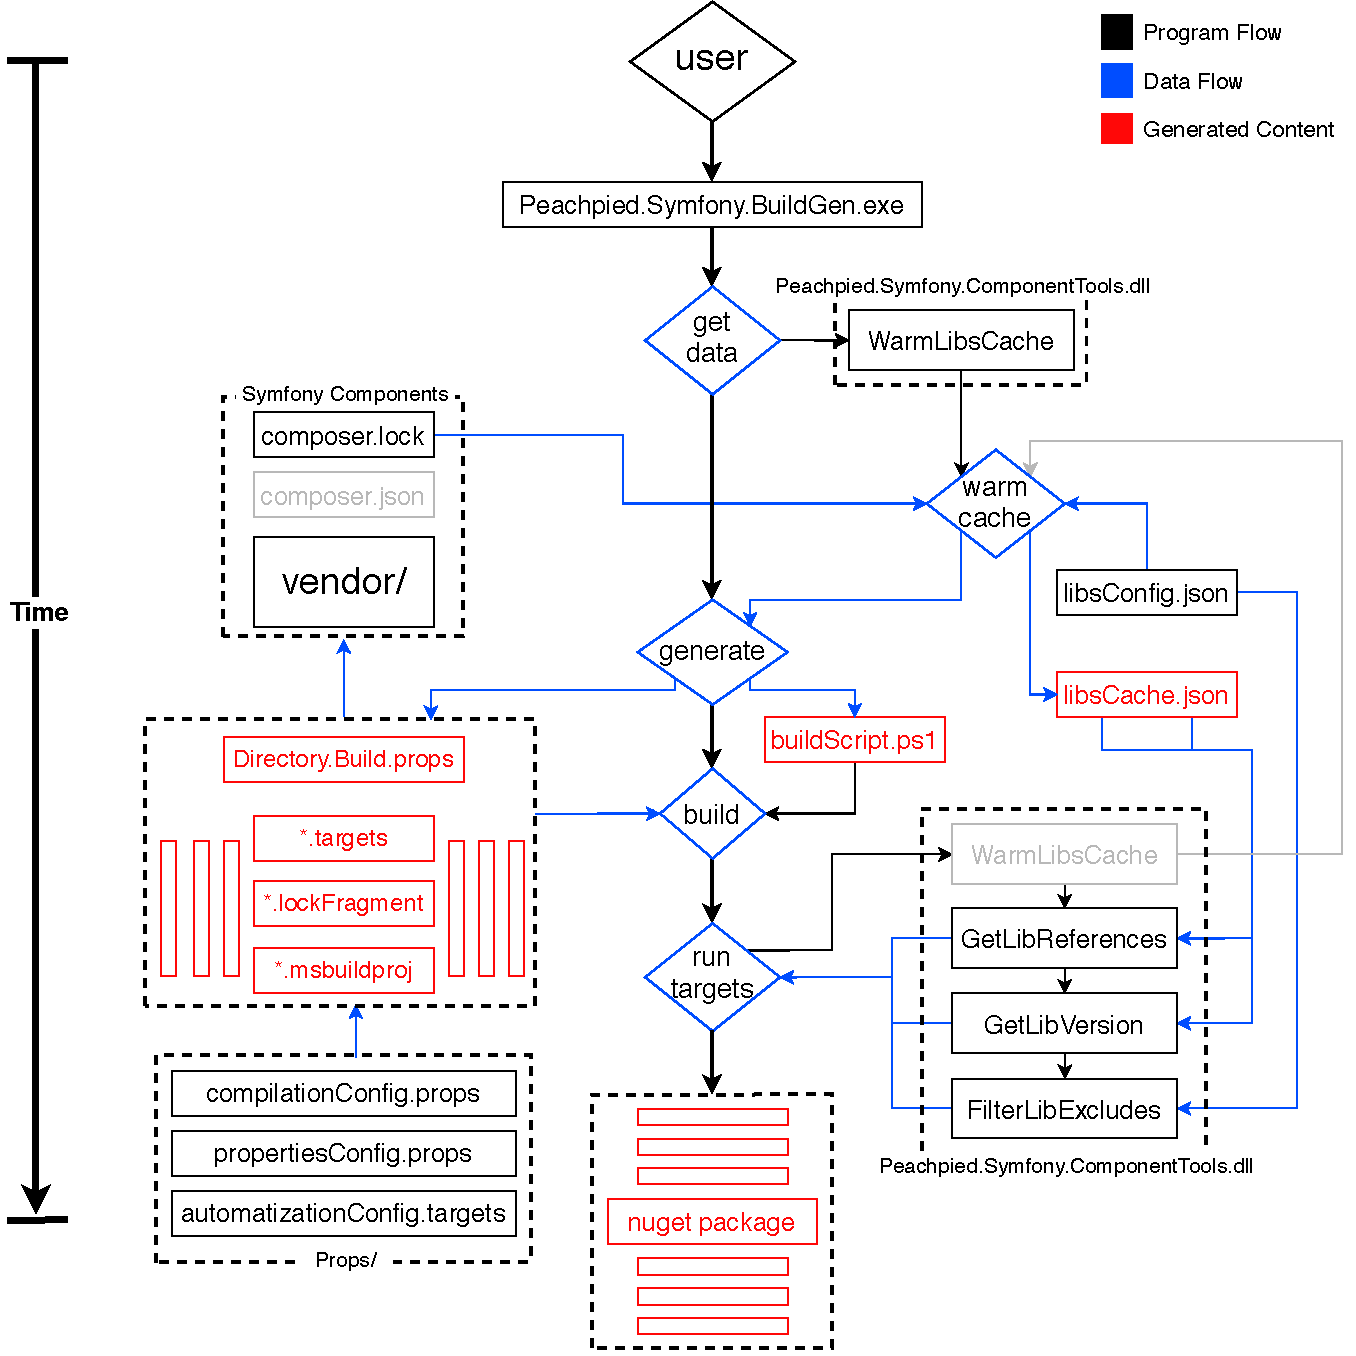
\includegraphics[width=\linewidth]{img/Components-compilation.pdf}
  \caption{Compilation process of Symfony components}
  \label{fig:Components-compilation}
\end{figure}


\paragraph{Peachpied.Symfony.BuildGen} This utility is distributed as an executable file that generates \texttt{.msbuildproj} and other necessary  files for every Symfony component found in the target directory. These are marked red in the Figure 5.1. In addition to, the utility also outputs the \texttt{buildScript.ps1} script that can be run in order to execute \texttt{dotnet build} on each produced \texttt{msbuildproj} in correct order. The target directory for the build generator is supplied by the \texttt{-p, --project} parameter. Aside from that, the utility also accepts optional paths to the \texttt{libsConfig.json} and \texttt{.props} files that are otherwise set to default values regarding the repository structure. Flag parameter \texttt{-b, --build} automatically runs generated \texttt{buildScript.ps1} on created files, and with the \texttt{-d, --debug} flag it is possible to skip final clean-up phase that automatically removes all generated files when the \texttt{-b} parameter is included.

List of Symfony Components present in the target directory is obtained using the \texttt{WarmLibsCache} class. This step is marked \texttt{\frenchspacing1.} and \texttt{\frenchspacing2.} in the Figure. In the step \texttt{\frenchspacing3.} of the Figure, we prepared public properties of the class with the help of \texttt{composer.lock} and \texttt{libsConfig.json} files. Load-up of these files is marked with the blue arrows leading towards the \texttt{warm cache} action in the Figure. As a side effect of the \texttt{WarmLibsCache} class execution, the \texttt{libsCache.json} file is produced for the obtained list of Symfony Components.

Step \texttt{\frenchspacing4.} of the Figure marks transfer to the generating phase of the compilation. Regarding the actual files provided by the build generator utility, it firstly creates the \texttt{Directory.Build.Props} file. After that, the necessary information like the list of package data and the ordered collection of package names are loaded from the \texttt{WarmLibsCache} class and one \texttt{[PackageName].msbuildproj}, one \texttt{[PackageName].lockFragment.json} or \texttt{[PackageName].lockFragment-dev.json}, and one \texttt{[PackageName].targets} file is generated for each Symfony Component. All generated files are placed in the target directory provided in order to comply previously mentioned requirement for paths to NuGet packages' static files.

The \texttt{.lockFragment} files hold each component's record parsed out from the \texttt{composer.lock} file. The \texttt{.targets} files are special as every NuGet package can include one such \texttt{.props} and \texttt{.targets} file that will be automatically imported into the project referring the NuGet. The requirements for this to work are to name the files accordingly to the package names and place them inside the \texttt{build} directory of the package. The files can be also copied to the \texttt{buildTransitive} directory which will result in transitive behaviour of the functionality. However, this feature is only available in NuGet version 5.0 and newer. Each \texttt{.targets} file provides a functionality to restore Symfony Component's folder inside the \texttt{vendor} directory of the project that uses the NuGet. In addition to, it also exposes the \texttt{LockFragments} item with appended path to its \texttt{.lockFragment.json} file. These functionalities are required for additional automation during actual Symfony project compilation and thus will be discussed in greater detail in the next chapter. A truncated example of one such \texttt{.targets} file can be found in the following Listing.

\begin{center}
\lstset{
	language=XML,
	morekeywords={encoding, version, xmlns, InitialTargets,
	Include, Condition, Name, Text, Importance, SourceFiles,
	DestinationFolder}}
\begin{lstlisting}[caption={Psr.Cache.targets},captionpos=b]
<?xml version="1.0" encoding="utf-8"?>
<Project xmlns="http://schemas.microsoft.com/developer/msbuild/2003" 
		InitialTargets="Copy_Psr_Cache_Vendor">
    
    <ItemGroup>
        <LockFragments Condition="{* file exists *}"
        		Include="{* package/build/ *}
        		../tools/any/any/Psr.Cache.lockFragment.json" />
        <LockFragments Condition="{* file exists *}"
        		Include="{* package/build/ *}
        		../tools/any/any/Psr.Cache.lockFragment-dev.json" />
    </ItemGroup>

    <Target Name="Copy_Psr_Cache_Vendor" 
    		Condition="$(RestoreVendor)==true 
 			AND {* project/vendor/psr/cache does not exist *}">
        <Message Text="Copying Psr.Cache assets..." Importance="high" />
        <ItemGroup>
            <Copy_Psr_Cache_Vendor_Files Include="{* package/build/ *}
            ../contentFiles/any/netcoreapp2.0/vendor/**/*.*" />
        </ItemGroup>
        <Copy SourceFiles="@(Copy_Psr_Cache_Vendor_Files)" 
        		DestinationFolder="{* project/vendor *}"/>
    </Target>

</Project>
\end{lstlisting}
\end{center}

Furthermore, with the use of previously mentioned ordered collection of package names, the \texttt{buildScript.ps1} file is generated providing means of automatic compilation of Symfony Components in the order denoted by the dependency tree. 

In case the \texttt{-b} flag was used, the utility next runs the \texttt{buildScript.ps1} script and proceeds to the compilation, marked with number \texttt{\frenchspacing5.} in the Figure. This is performed as described in the previous sections. First, the \texttt{.msbuidproj} file is loaded. After that, MSBuild targets run in execution order and handle importing of \texttt{.props} with \texttt{automatizationConfig.targets} and ultimately locating package specific \texttt{lockFragments} and \texttt{.targets} as well. Figure 5.1 depicts this phase separated from automatization targets execution in sake of increased readability. During the MSBuild targets execution named the \texttt{run targets} action in the Figure 5.1, custom targets are executed chronologically in displayed order providing missing information for the compilation and optionally skipping the \texttt{WarmLibsCache} target in case the \texttt{libsCache.json} file is already present in the target directory. This corresponds to the steps \texttt{\frenchspacing6.} to \texttt{\frenchspacing10.} in the Figure and on completion, passes control back to the MSBuild targets that finally produce NuGet packages.

We can now sum-up the actual compilation process of a set of Symfony components from the earliest phase of PHP sources downloading to producing actual NuGet packages into the following steps.

\begin{enumerate}[i:]
\item Clone the repository and initialize a directory under the \texttt{Peachpied.Symfony/Components} path with the \texttt{composer init} command (optionally skip the interactive \texttt{composer.json} configuration).
\item Require a set of Symfony components either by running \texttt{composer require [packageName:version]} or in the interactive configuration during the previous step.
\item Compile the \texttt{Peachpied.Symfony.BuildGen} sources with the \texttt{dotnet publish -r {Runtime}} command into executable file.
\item Run the build generator tool supplying the path to the target directory.
\item Modify sources uncompilable by the compiler and extend the \texttt{libsConfig.json} file with an additional configuration for problematic packages if needed.
\item Find the produced NuGet packages under the \texttt{Nuget-Repository/Components} path.
\end{enumerate}

Finally, one can notice that to compile Symfony components of an existing Symfony project first two steps will not probably need to be executed. The third step is also a one time job, and the fifth step should not be needed when Peachpie compiler is ready for the production and when the \texttt{libsConfig.json} contains all the necessary configurations after supplied by the community. Therefore, the whole compilation would in such case reduce to a single step of manual execution of the build generator tool. This can be observed on the Figure 5.1 where the execution of the tool is followed by automatic actions all the way to the NuGet packages producing.
